\documentclass[border=4pt]{standalone}

% --- packages (mirror these in loss.meta.json "requires") ---
\usepackage{tikz}
\usetikzlibrary{arrows.meta}

% --- palette (canonical source: reference/color-palettes/color-palettes.md; light variant) ---
\definecolor{otblue}{HTML}{0072B2}
\definecolor{otorange}{HTML}{E69F00}
\definecolor{otteal}{HTML}{009E73}
\definecolor{otpurple}{HTML}{CC79A7}
\definecolor{otgray}{HTML}{5A5A5A}

\begin{document}
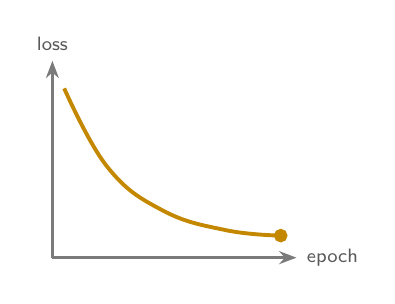
\begin{tikzpicture}[line width=0.9pt, >={Stealth[length=2.2mm]}]
  % axes
  \draw[->, otgray!80] (0,0) -- (3.1,0) node[right, font=\sffamily\scriptsize, text=otgray] {epoch};
  \draw[->, otgray!80] (0,0) -- (0,2.5) node[above, font=\sffamily\scriptsize, text=otgray] {loss};
  % descending loss curve
  \draw[otorange!85!black, line width=1.4pt]
    plot[smooth, tension=0.7] coordinates {(0.15,2.15) (0.7,1.15) (1.4,0.6) (2.2,0.35) (2.9,0.28)};
  % converged minimum
  \filldraw[otorange!85!black] (2.9,0.28) circle[radius=0.07];
\end{tikzpicture}
\end{document}
